\documentclass[10pt, aspectratio=169]{beamer}
\usepackage{tabularx}
\usepackage{booktabs}
\usepackage{graphicx}

\usetheme{Goettingen}
\usecolortheme{seahorse}
\usepackage{tikz}
\usetikzlibrary{shapes.geometric, arrows}
\usepackage{hyperref}
%\useoutertheme{miniframes} % Alternatively: miniframes, infolines, split
\useinnertheme{circles}
\usetikzlibrary{fit}
\usepackage{wrapfig}
\usepackage{pgfplots}
\pgfplotsset{compat=1.18}
\usepackage{pgfplotstable}
\usepackage{outlines}
\usepackage{algorithm}
\usepackage{algorithmicx}
\usepackage{algpseudocode}
\usepackage{amsmath}
\usepackage[numbers]{natbib}
\usepackage{cite}
\usepackage{caption}
\usepackage{colortbl} 
\usepackage{xcolor}
\setbeamertemplate{itemize item}[circle] % Level 1 bullets
\setbeamertemplate{itemize subitem}[square] % Level 2 bullets
\setbeamertemplate{itemize subsubitem}[triangle] % Level 3 bullets

\titlegraphic{
    
\includegraphics[width=1.55cm]{img/logo copy.png}
    }
    \title{Music Genre Classification Using Multiple Classifiers} 
    \subtitle{Machine Learning Project}
    \subject{Random Forests}
    \author{Lisa Korntheuer, Jan Birkert, Adrian Desiderato, Jan Wangerin, Spyridon Spyropoulos}
    \institute{Technische Hochschule Ulm}
    \date{\today}
    \logo{
        
\includegraphics[width=1.55cm]{img/logo copy.png}
        }
        %\setbeamercolor{subsection in head/foot}{bg=UBCgrey,fg=white}
        \setbeamertemplate{footline}[frame number]
        \AtBeginSection[]{%
        \setbeamertemplate{footline}{}
        \begin{frame}[noframenumbering]
            \frametitle{Table of Contents}
            \tableofcontents[currentsection]
        \end{frame}
        \setbeamertemplate{footline}[frame number]
        }
\begin{document}

\newcommand{\subtext}[1]{$_{\text{#1}}$}

\begin{frame}
    \maketitle
\end{frame}
\setbeamertemplate{footline}{}
\begin{frame}[noframenumbering]
    \frametitle{Table of Contents}
    \tableofcontents
\end{frame}
\AtBeginSection[]{
        }
        \setbeamertemplate{footline}[frame number]
\section{Introduction}
\begin{frame}
    \frametitle{Introduction}
    \begin{outline}
        \1 This is an awesome slide with very important information. 
    \end{outline}
\end{frame}
\AtBeginSection[]{%
        \setbeamertemplate{footline}{}
        \begin{frame}[noframenumbering]
            \frametitle{Table of Contents}
            \tableofcontents[currentsection]
        \end{frame}
        \setbeamertemplate{footline}[frame number]
        }

\section{Data Understanding}
\begin{frame}
    \frametitle{Data Understanding}
    \begin{outline}
        \1 This is an awesome slide with very important information. 
    \end{outline}

\end{frame}
\section{Data Preparation}
\begin{frame}
    \frametitle{Data Preparation}
    \begin{outline}
        \1 This is an awesome slide with very important information. 
    \end{outline}
\end{frame}
\section{Modeling}
\subsection{Random Forest}
\begin{frame}
    \frametitle{Modeling --- Random Forest}
    \begin{itemize}
        \item Two experimenting approaches using GridSearchCV:
        \begin{itemize}
            \item Soft hyperparameter tuning:
            \begin{itemize}
                \item Number of trees (default = 100)
                \item Splitting criterion (default = Gini)
            \end{itemize}
            \item Heavy hyperparameter tuning:
            \begin{itemize}
                \item Number of trees (default = 100)
                \item Splitting criterion (default = Gini)
                \item Maximum depth (default = None)
                \item Minimum samples per leaf (default = 1)
                \item Minimum samples per split (default = 2)
                \item Maximum features (default = sqrt)
            \end{itemize}
        \end{itemize}
    \end{itemize}
\end{frame}

\begin{frame}
    \frametitle{Modeling --- Random Forest: Results}
    \begin{itemize}
        \item Soft hyperparameter tuning:
        \begin{itemize}
            \item Training time: 20s
            \item Accuracy: 0.760
            \item Parameters: Number of trees = 1000, Splitting criterion = Gini
        \end{itemize}
        \item Heavy hyperparameter tuning:
        \begin{itemize}
            \item Training time: 18min
            \item Accuracy: 0.760
            \item Parameters: Exactly the same forest as in the soft hyperparameter tuning
        \end{itemize}
    \end{itemize}
\end{frame}

\subsection{Decision Trees}
\begin{frame}
    \frametitle{Modeling --- Decision Trees}
    \begin{outline}
        \1 This is an awesome slide with very important information. 
    \end{outline}
\end{frame}

\subsection{K-Nearest-Neighbors}
\begin{frame}
    \frametitle{Modeling --- K-Nearest-Neighbors}
    \textbf{Hyperparameter tuning} of 3 selected parameters with \textit{GridSearchCV}:
    \begin{itemize}
        \item \textbf{n\_neighbors} : number of neighbors $k$
        \item \textbf{weights} : weights assigned to the nearest neighbors
            \begin{itemize} 
                \item 'uniform'
                \item 'distance'
            \end{itemize}
        \item \textbf{metric} : method for distance computation
            \begin{itemize}
                \item 'euclidean'
                \item 'manhattan'
            \end{itemize}
    \end{itemize}
\end{frame}
\begin{frame}
    \frametitle{Modeling --- K-Nearest-Neighbors: Results}
    \begin{itemize}
        \item \textbf{Optimal parameter set:}
            \begin{itemize}
                \item $k=3$ nearest neighbors
                \item distance-dependent weights
                \item Manhattan distance
            \end{itemize}
            Remark: Distance-dependent weights might lead to overfitting
        \item \textbf{Test accuracy:} 0.74
    \end{itemize}
\end{frame}

\subsection{Artificial Neural Network}
\begin{frame}
    \frametitle{Modeling --- Artificial Neural Network}
    \begin{outline}
        \1 Goal: Find the \textbf{best combination of hyperparameter values} to train a \textbf{Multilayer Perceptron} model
        \1 The \textbf{following hyperparameters} were examined by means of a \textbf{Randomized Search Cross Validation}:
            \2 Two hidden layers with random number of neurons $\in[2, 200]$
            \2 The activation functions \texttt{tanh}, \texttt{relu} or \texttt{logistic}
            \2 $\alpha$-values of either $0.0001$, $0.001$ or $0.05$
            \2 A random learning rate $\in[0.001, 0.01]$
            \2 A batch size $\in[16, 128]$
            \2 \texttt{constant}, \texttt{adaptive} and \texttt{invscaling} learning rates were tested
        \1 Cross Validation was run with \textbf{10 folds}
    \end{outline}   
\end{frame}
\begin{frame}{Modeling --- Artificial Neural Network: Results}
    \begin{outline}
        \1 After running the hyperparameter tuning \textbf{10 times}, our best result was:
            \2 Two hidden layers with random number of neurons $\in[2, 200]$
            \2 The activation functions \texttt{tanh}, \texttt{relu} or \texttt{logistic}
            \2 $\alpha$-value of $0.001$
            \2 A random learning rate of $\sim 0.0014$
            \2 A batch size of $63$
            \2 An \texttt{invscaling} learning rate
        \1 With these parameters, we achieved a \textbf{train accuracy of $\mathbf{97.25\%}$} and a \textbf{test accuracy of $\mathbf{77.0\%}$}
        \1 \textbf{Remarks:}
            \2 \textit{We also tested with a third hidden layer without improvement}
            \2 Additionally, we also tried the \texttt{lbfgs} activation function which led to way worse results
    \end{outline}
\end{frame}

\section{Evaluation}
\subsection{Comparison}
\begin{frame}
    \frametitle{Comparison --- Results}
    \begin{table}[h!]
        \centering
        \begin{tabular}{|l|c|c|c|}
        \hline
        \textbf{Model}         & \textbf{Accuracy} & \textbf{F1 Score } & \textbf{ROC AUC } \\ \hline
        MLP                    & 0.770             & 0.772                       & 0.956                   \\ \hline
        Random Forest          & 0.760             & 0.761                       & 0.958                   \\ \hline
        KNN                    & 0.740             & 0.743                       & 0.913                   \\ \hline
        Decision Tree          & 0.530             & 0.532                       & 0.759                   \\ \hline
       
        
        \end{tabular}
        \caption{Model performance comparison.}
        \label{tab:model_performance}
        \end{table}

\end{frame}
\begin{frame}
    \frametitle{Comparison --- ROC Curves}
    \begin{figure}
        \centering
        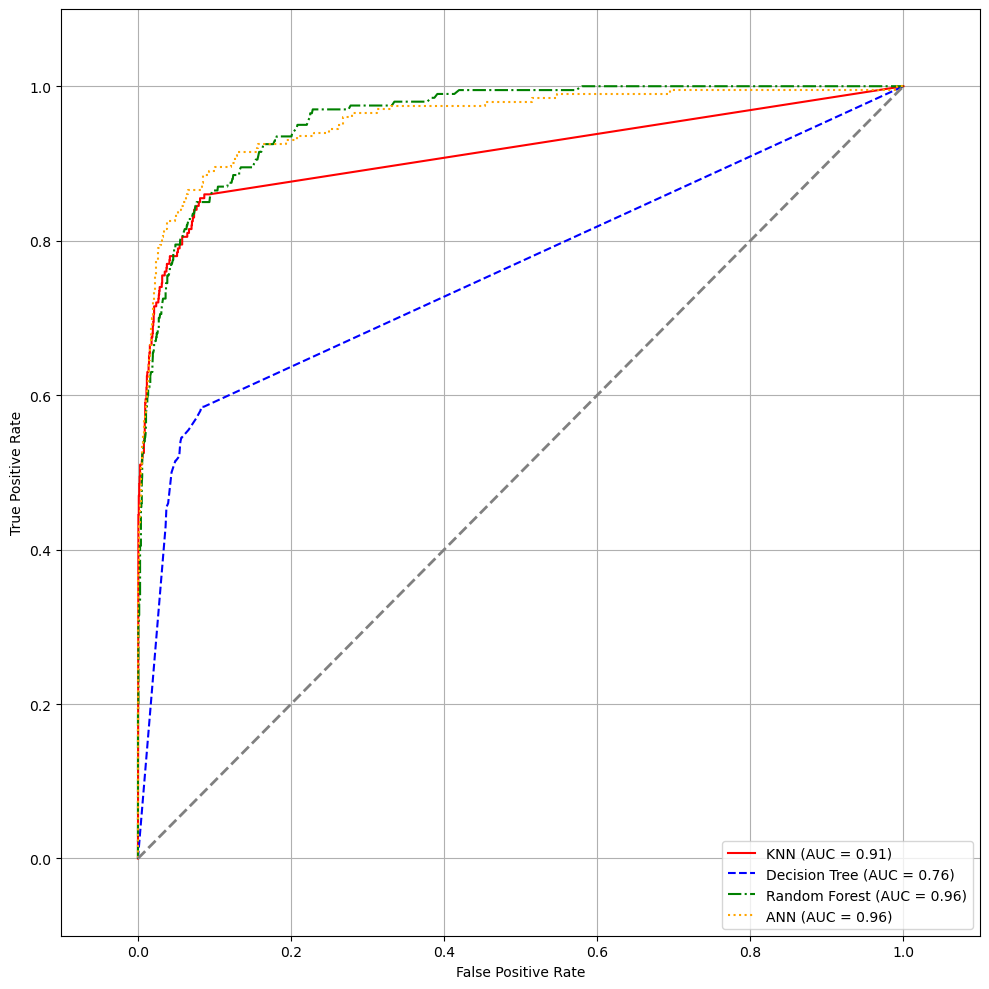
\includegraphics[width=0.44\textwidth]{img/roc.png}
        \caption{ROC Curves of the different classifiers}
    \end{figure}
\end{frame}
\subsection{Experimentation}
\begin{frame}
    \frametitle{Experimentation --- 13 Datapoints}
    
    \begin{table}[h!]
        \centering
        \resizebox{12cm}{3.3cm}{
        \begin{tabular}{|c|l|l|l|l|l|}
        \hline
        \textbf{Datapoint} & \textbf{True Label} & \textbf{Random Forest Prediction} & \textbf{KNN Prediction} & \textbf{Decision Tree Prediction} & \textbf{ANN Prediction} \\ \hline
        0                  & pop                 & \cellcolor{red!30}hiphop          & \cellcolor{red!30}hiphop & \cellcolor{red!30}hiphop          & \cellcolor{red!30}blues \\ \hline
        1                  & pop                 & \cellcolor{red!30}hiphop          & \cellcolor{red!30}hiphop & \cellcolor{red!30}disco           & \cellcolor{red!30}hiphop \\ \hline
        2                  & pop                 & \cellcolor{red!30}hiphop          & \cellcolor{red!30}hiphop & \cellcolor{red!30}hiphop          & \cellcolor{red!30}hiphop \\ \hline
        3                  & metal               & \cellcolor{red!30}hiphop          & \cellcolor{red!30}hiphop & \cellcolor{red!30}hiphop          & \cellcolor{red!30}blues \\ \hline
        4                  & metal               & \cellcolor{red!30}hiphop          & \cellcolor{red!30}blues  & \cellcolor{red!30}hiphop          & \cellcolor{red!30}hiphop \\ \hline
        5                  & blues               & \cellcolor{green!30}blues         & \cellcolor{green!30}blues & \cellcolor{red!30}disco           & \cellcolor{green!30}blues \\ \hline
        6                  & blues               & \cellcolor{green!30}blues         & \cellcolor{green!30}blues & \cellcolor{red!30}country         & \cellcolor{red!30}hiphop \\ \hline
        7                  & blues               & \cellcolor{red!30}hiphop          & \cellcolor{red!30}reggae & \cellcolor{red!30}hiphop          & \cellcolor{red!30}reggae \\ \hline
        8                  & classical           & \cellcolor{red!30}jazz            & \cellcolor{red!30}jazz   & \cellcolor{red!30}disco           & \cellcolor{red!30}hiphop \\ \hline
        9                  & classical           & \cellcolor{red!30}jazz            & \cellcolor{red!30}jazz   & \cellcolor{red!30}country         & \cellcolor{red!30}blues \\ \hline
        10                 & classical           & \cellcolor{red!30}jazz            & \cellcolor{red!30}jazz   & \cellcolor{red!30}jazz            & \cellcolor{red!30}hiphop \\ \hline
        11                 & rock                & \cellcolor{red!30}hiphop          & \cellcolor{red!30}hiphop & \cellcolor{red!30}hiphop          & \cellcolor{red!30}reggae \\ \hline
        12                 & rock                & \cellcolor{red!30}hiphop          & \cellcolor{red!30}blues  & \cellcolor{red!30}hiphop          & \cellcolor{red!30}hiphop \\ \hline
        13                 & rock                & \cellcolor{red!30}hiphop          & \cellcolor{red!30}reggae & \cellcolor{red!30}hiphop          & \cellcolor{red!30}reggae \\ \hline
        \end{tabular}
}
        \caption{Comparison of predictions from Random Forest, KNN, Decision Tree, and ANN against true labels.}
        \label{tab:model_predictions}
        \end{table}
\end{frame}
\section{Conclusion}
\begin{frame}
    \frametitle{Conclusion}
    \begin{outline}
        \1 Each classifier (KNN, Decision Tree, Random Forest, ANN) had different trade-offs
        \1 Decision Trees performed poorly, even with pruning
        \1 Random Forest and ANN showed strong performance
            \2 ANN with best accuracy ($\sim 77\%$)
            \2 kNN showed surprisingly good results
        \1 Random Forests, ANNs, and kNNs are suitable for music classification
            \2 However: $\sim 25\%$ of predictions may be incorrect
        \1 Practical example with own tracks showed poor accuracy
    \end{outline}
\end{frame}
\setbeamertemplate{footline}{}
\begin{frame}[noframenumbering]
    \frametitle{References}
    {\tiny\bibliography{references.bib}
    \bibliographystyle{IEEEtranN}
    \nocite{*}}
\end{frame}

\end{document}